\documentclass{article}

\title{Candid for engineers}
\subtitle{A practical guide to the world's most advanced interface definition language.}
\date{2023-06-14}
\modified{2023-06-22}

\keyword{ic}

\begin{document}
\section{introduction}{Introduction}

\href{https://github.com/dfinity/candid}{Candid} is the primary interface definition language for smart contracts hosted on the \href{https://internetcomputer.org/}{Internet Computer}.

Most prevalent data-interchange formats, such as \href{https://protobuf.dev/}{Protocol Buffers} and \href{https://thrift.apache.org/}{Thrift}, come straight from \href{https://reasonablypolymorphic.com/blog/protos-are-wrong/#ad-hoc-and-built-by-amateurs}{engineering departments}.

Candid is different.
Candid is a child of programming language designers who grew it from \href{https://github.com/dfinity/candid/blob/master/spec/Candid.md#design-goals}{first principles}.
As a result, Candid \href{https://github.com/dfinity/candid/blob/master/spec/IDL-Soundness.md}{makes sense} but might feel alien to most engineers.

This article is an introduction to Candid I wish I had when I started using it.

\section{candid-overview}{Candid overview}

As any interface definition language, Candid has multiple facets.

One facet is the textual format defining the service interface.
This facet is similar in function to the \href{https://grpc.io/}{gRPC} system.
Another facet is the binary format for encoding service requests and responses.
This facet is analogous to the \href{https://protobuf.dev/}{Protocol Buffers} serialization format.

Though Candid is similar to gRPC on the surface, there is an essential distinction between the two systems.

gRPC builds strictly on top of the Protocol Buffers format.
Service method definitions can refer to message definitions, but messages cannot refer to services.

Candid, on the other hand, ties the message format and service definition language into a knot.
Service method definitions can refer to data types, and data types can refer to services.
Services can accept as arguments and return references to other services and methods.
The Candid team usually calls such designs ``higher-order cases''.
The \href{https://internetcomputer.org/docs/current/developer-docs/backend/candid/candid-concepts}{Candid overview} article introduces a higher-order function in its first example.

\begin{figure}
\begin{code}[candid]
\b{service} counter : {
  \em{// A method taking a reference to a function.}
  subscribe : (func (int) -> ()) -> ();
}
\end{code}
\end{figure}

Another distinctive Candid feature is \href{#subtyping}{subtyping rules} for defining backward-compatible service evolution.
That's when you want formal language designers on your team.

\subsection{service-definitions}{Service definitions}

Most often, developers interact with Candid through the service definition files, also known as \href{https://internetcomputer.org/docs/current/developer-docs/backend/candid/candid-howto#the-did-file}{\code{.did}} files.

A \code{.did} file contains type definitions and at most one primary service definition, which must be the last clause in the \code{.did} file.

\begin{figure}
\marginnote{mn-token-interface}{
    The definition of a token ledger registry service.
    The \code{service} keyword at the top level defines the primary service; it must appear as the last definition in the file.
    Note the difference between a service type definition (top) and a service definition (bottom) syntactic forms.
}
\begin{code}[candid]
// A type definition introducing the Token service interface.
\b{type} Token = \b{service} {
  token_symbol : () -> (text) query;
  balance : (record { of : principal }) -> (nat) query;
  transfer : (record { to : principal; amount : nat }) -> ();
};

\b{service} TokenRegistry : {
  \em{// Returns a reference to a token ledger service given the token symbol.}
  lookup : (symbol : text) -> (opt Token) query;
}
\end{code}
\end{figure}

Two syntactic forms can introduce a service definition: with and without init arguments.
The technical term for a service definition with init arguments is \href{https://github.com/dfinity/candid/blob/master/spec/Candid.md#services}{service constructor}\sidenote{sn-class}{
    Some implementations use the term \href{https://docs.rs/candid/0.8.4/candid/types/internal/enum.Type.html#variant.Class}{\em{class}}.
}

\begin{figure}
\marginnote{mn-service-vs-constructor}{
  Service definitions with (top) and without (bottom) init arguments (rendered in bold font).
}
\begin{code}[candid]
\b{service} Token : {
  balance : (record { of : principal }) -> (nat) query;
  \em{// ...}
}
\end{code}
\begin{code}[candid]
\b{service} Token : \b{(init_balances : vec record \{ principal; nat \})} -> {
  balance : (record { of : principal }) -> (nat) query;
  \em{// ...}
}
\end{code}
\end{figure}

Conceptually, a service constructor represents an uninitialized canister, whereas a service represents a deployed canister.
Init arguments describe the value the canister maintainers must specify when instantiating the canister.

Ideally, canister \em{build} tools should produce a \b{service constructor}.
If the module contains no init args, the tools should use the form \code{service : () -> \{\ldots\}}.
Canister \em{deploy} tools, such as \href{https://internetcomputer.org/docs/current/references/cli-reference/dfx-deploy}{\code{dfx deploy}}, should use the init args to install the canister, and use the \b{service} as the public metadata, stripping out the init args.
As of July 2023, Motoko compiler and Rust CDK don't follow these conventions, so people often conflate the two concepts.

\subsection{types}{Types}

In addition to a rich set of primitive types, such as booleans (\code{bool}), floats (\code{float64}), strings (\code{text}), and whole numbers of various widths (\code{nat8}, \code{nat16}, \code{nat32}, \code{nat64}, \code{int8}, \code{int16}, \code{int32}, \code{int64}), Candid provides a few more advanced types and type constructors:

\begin{itemize}
    \item
    Arbitrary-precision integers (\href{https://internetcomputer.org/docs/current/references/candid-ref#type-nat}{\code{nat}} and \href{https://internetcomputer.org/docs/current/references/candid-ref#type-int}{\code{int}}).
    \item
    Unique identifiers (\href{https://internetcomputer.org/docs/current/references/candid-ref#type-principal}{\code{principal}}).
    \item
    The \href{https://internetcomputer.org/docs/current/references/candid-ref#type-opt-t}{\code{opt}} type constructor for marking values as potentially missing.
    \item
    The \href{https://internetcomputer.org/docs/current/references/candid-ref#type-vec-t}{\code{vec}} type constructor for declaring collections.
    \item
    \href{https://internetcomputer.org/docs/current/references/candid-ref#type-record--n--t--}{Records} as product types (also known as \code{structs}) with named fields, such as \newline
    \code{\b{record} \{ \em{first_line} : text; \em{second_line} : \b{opt} text; \em{zip} : text; /* \ldots  */ \}}.
    \item
    \href{https://internetcomputer.org/docs/current/references/candid-ref#type-variant--n--t--}{Variants} as sum types (also known as \code{enums}) with named alternatives, such as \newline
    \code{\b{variant} \{ \em{cash}; \em{credit_card} : \b{record} \{ /* \ldots  */ \} \}}.
    \item
    The \href{https://internetcomputer.org/docs/current/references/candid-ref#type-reserved}{\code{reserved}} type for retiring unused fields.
    \item
    The \href{https://internetcomputer.org/docs/current/references/candid-ref#type-empty}{\code{empty}} that has no constructors.
    It might be helpful for marking some alternatives as impossible, for example, \code{variant \{ Ok : int; Err : empty \}}.
    \item
    The \href{https://internetcomputer.org/docs/current/references/candid-ref#type-null}{\code{null}} type (also known as the \href{https://en.wikipedia.org/wiki/Unit_type}{unit type}) containing a single value, \code{null}.
    You use it implicitly every time you define variant alternatives not containing any data.
    For example, \code{variant \{ A; B \}} and \code{variant \{ A : null; B : null \}} are equivalent types.
    \item
    The \href{https://internetcomputer.org/docs/current/references/candid-ref#type-func---}{\code{func}} type family describing actor method signatures.
    Values of such types represent references to actor methods (actor address + method) of the corresponding type.
    \item
    The \href{https://internetcomputer.org/docs/current/references/candid-ref#type-service-}{\code{service}} type family describing actor interfaces.
    It might be helpful to view a service type as a special kind of record where all fields are functions.
    Values of service types represent references to actors providing the corresponding interface.
\end{itemize}

Candid also allows recursive and mutually-recursive types.

\begin{code}[good]
type tree = variant { leaf : nat; children : forest };
type forest = vec tree;
\end{code}

\subsection{records-and-variants}{Records and variants}

Records and variants are the bread and butter of working with Candid.

Records and variants have similar syntax; the primary difference is the keyword introducing the type.
The meanings of the constructs are complementary, however.
A record type indicates that \em{all} of its fields must be set, and a variant type indicates that precisely \em{one} field must be set.

\begin{figure}
\marginnote{mn-record-vs-variant}{
 Record and variant definitions have similar syntax but different semantics.
 In a record, all fields must be set.
 In a variant, precisely one alternative must be set.
}

\begin{code}[candid]
\b{type} Employee = \b{record} {
  first_name : text;
  second_name : text;
  status : EmployeeStatus;
};

\b{type} EmployeeStatus = \b{variant} {
  full_time;
  contractor : record { contract_expires_at : opt nat };
};
\end{code}
\end{figure}

Similarly to Protocol Buffers, Candid uses integers to identify fields and alternatives.
Unlike Protocol Buffers, Candid doesn't ask the programmer to map symbolic field names to integers, relying on a \href{https://github.com/dfinity/candid/blob/master/spec/Candid.md#shorthand-symbolic-field-ids}{hash function} instead.
This design choice has two practical implications.

\begin{itemize}
    \item
    Renaming a field or an alternative is a backward-incompatible change.
    \item
    Tools cannot display field names without the service definition file.
\end{itemize}

Please refer to the \href{https://www.joachim-breitner.de/blog/786-A_Candid_explainer__Quirks#hashed-field-names}{hashed field names} section in Joachim's article for more insight and references.

\subsection{tuples}{Tuples}

Candid doesn't provide first-class tuples.
There are two constructs closely resembling tuples, however.

\begin{enumerate}
    \item
    Records with \href{https://github.com/dfinity/candid/blob/master/spec/Candid.md#shorthand-tuple-fields}{omitted field names} act as type-level tuples.
    Candid language integrations, such as \href{https://internetcomputer.org/docs/current/developer-docs/backend/candid/candid-howto#interact-with-a-service-from-a-motoko-canister}{native Motoko support} and Rust \href{https://crates.io/crates/candid}{candid} package, use this feature to map native tuples to Candid.
    \item
    Argument and result sequences in service methods behave a lot like tuples.
\end{enumerate}

\begin{figure}
\marginnote{mn-tuple-like}{
  Tuple-like constructions in Candid: a record with tuple fields (top) and argument sequences (bottom).
}
\begin{code}[candid]
\em{// A record with tuple fields.}
\b{type} Entry  = \b{record} { text; nat };
\em{// The Entry and ExplicitEntry types are equivalent.}
\b{type} ExplicitEntry = \b{record} { \b{0} : text; \b{1} : nat };

service ArithmeticService : {
  \em{// Argument and result sequences.}
  div : (divident : nat, divisor : nat) -> (quotient : nat, reminder : nat) query;
}
\end{code}
\end{figure}

Note that Candid ignores argument and result names in method signatures; it relies solely on the argument position within the sequence.
Extending the argument sequence with a new optional value is safe, but adding an argument in the middle will break backward compatibility.
Prefer using records as arguments and result types: you'll have more freedom to rearrange or remove fields as the interface evolves.

\begin{figure}
\marginnote{mn-record-in-args}{
  Using records with named fields as method arguments and results.
}
\begin{code}[candid]
service ArithmeticService : {
  div : (record { divident : nat; divisor : nat })
     -> (record { quotient : nat; reminder : nat }) query;
}
\end{code}
\end{figure}

See the \href{https://www.joachim-breitner.de/blog/786-A_Candid_explainer__Quirks#tuples}{Tuples} section in Joachim's article for more detail and advice.

\subsection{structural-typing}{Structural typing}

Candid's type system is \href{https://en.wikipedia.org/wiki/Structural_type_system}{structural}: it treats types as equal if they have the same structure.
Type names serve as monikers for the type structure, not as the type's identity.

Variable bindings in Rust are a good analogy for type names in Candid.
The \code{let x = 5;} statement \em{binds} name \em{x} to value \code{5}, but \em{x} does not become the identity of that value.
Expressions such as \code{x == 5} and \code{\{ let y = 5; y == x \}} evaluate to \code{true}.

\begin{figure}
\marginnote{mn-structural-types}{
  Candid views types \code{Point2d}, modeling a point on a plane, and \code{ECPoint}, modeling a point on an elliptic curve, as interchangeable because they have the same structure.
}

\begin{code}[candid]
\em{// These types are identical from Candid's point of view.}
type Point2d = record { x : int; y : int };
type ECPoint = record { x : int; y : int };
\end{code}
\end{figure}

Usually, you don't have to name types; you can inline them in service definitions (unless you define recursive types, of course).
Assigning descriptive names can improve the interface readability, however.

\begin{figure}
\marginnote{mn-type-names}{
  Candid allows you to omit type names for non-recursive type definitions.
  Service types \code{S1} and \code{S2} are interchangeable.
}

\begin{code}[candid]
type \b{S1} = service {
  store_profile : (nat, record { name : text; age : nat }) -> ();
};

type UserProfile = record { name : text; age : nat };
type UserId = nat;

type \b{S2} = service {
  store_profile : (UserId, UserProfile) -> ();
};
\end{code}
\end{figure}

\subsection{subtyping}{Subtyping}

One of Candid's distinctive traits is the use of structural \href{https://en.wikipedia.org/wiki/Subtyping}{subtyping} for defining backward-compatible interface evolutions\sidenote{sn-upgradable}{
  The Candid spec calls such evolutions \href{https://github.com/dfinity/candid/blob/master/spec/Candid.md#upgrading-and-subtyping}{type upgrades}.
}.
If a type \math{T} is a subtype of type \math{V} (denoted \math{T <: V}), then Candid can decode any value of type \math{T} into a value of type \math{V}.

Let's inspect some of the basic subtyping rules for simple values (not functions):

\begin{itemize}
    \item
    Subtyping is \href{https://en.wikipedia.org/wiki/Reflexive_relation}{reflexive}: any type is a subtype of itself.
    You can't break the clients if you don't change the interface.
    \item
    Subtyping is \href{https://en.wikipedia.org/wiki/Transitive_relation}{transitive}: \math{T <: V} and \math{V <: W} implies \math{T <: W}.
    A sequence of backward-compatible changes is backward-compatible.
    \item
    Adding a new field to a record creates a subtype.\newline
    \code{record \{ name : text; status : variant \{ user; admin \} \} <: record \{ name : text \} }
    \item
    Less intuitively, removing an \em{optional} field also creates a subtype.
    \newline
    \code{record \{ name : text \} <: record \{ name : text; status : \b{opt} variant \{ user; admin \} \} }
    \item
    Removing a case in a variant creates a subtype.\newline
    \code{variant \{ yes; no \} <: variant \{ yes; no; unknown \}}
    \item
    All types are subtypes of the \code{reserved} type.
    Candid will happily decode any type into a reserved field.
\end{itemize}

Function subtyping follows the standard \href{https://en.wikipedia.org/wiki/Covariance_and_contravariance_(computer_science)#Function_types}{variance rules}:
function \code{g : C -> D} is a subtype of function \code{f : A -> B} if \code{A <: C} and \code{D <: B}.
Informally, \code{g} must accept the same or more generic arguments as \code{f} and produce the same or more specific results as \code{f}.

\begin{figure}[grayscale-diagram]
\marginnote{mn-function-variance}{
  Function subtyping rules.
  As the interface evolves, the input types become more general, while output types become more restricted.
}
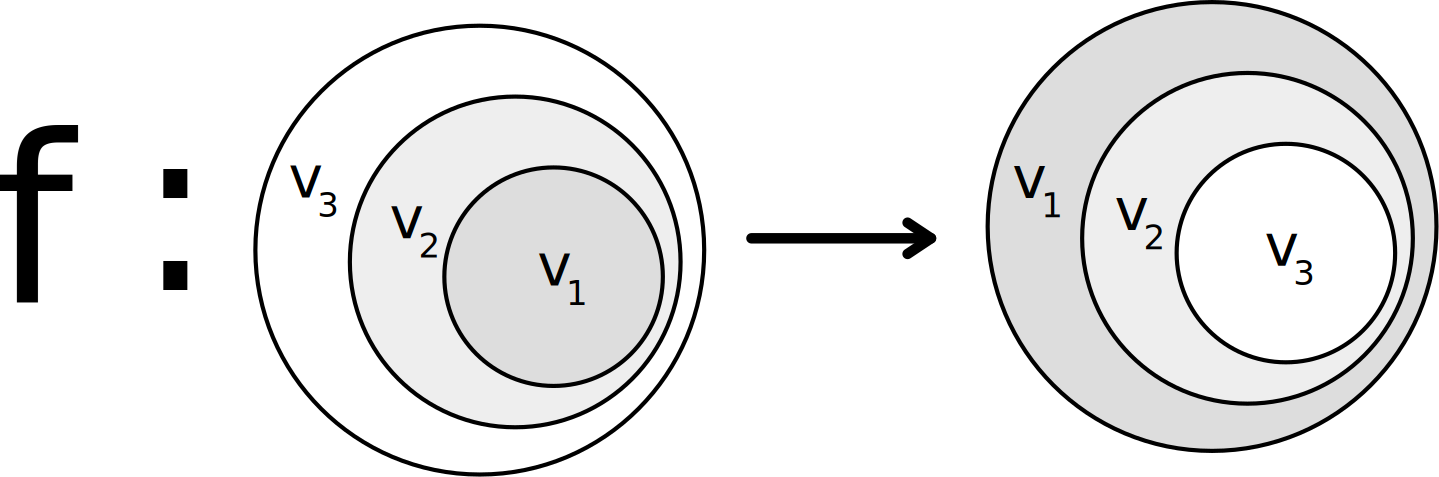
\includegraphics{/images/20-function-variance.svg}
\end{figure}

The rules mentioned in this section are by no means complete or precise; please refer to the \href{https://github.com/dfinity/candid/blob/master/spec/Candid.md#rules}{typing rules} section of the Candid specification for a formal definition.

Understanding the subtyping rules for functions is helpful for reasoning about safe interface migrations.
Let's consider a few examples of common changes that preserve backward compatibility of a function interface (note that compatibility rules for arguments and results are often reversed).

\begin{itemize}
    \item
    Remove an unused record field (or, better, change its type to \code{reserved}) from the method \em{input} argument.
    \item
    Add a new case to a variant in the method \em{input} argument.
    \item
    Add a new field to a record in the method \em{result} type.
    \item
    Remove an optional field from a record in the method \em{result} type.
    \item
    Remove an alternative from a variant type in the method \em{result} type.
\end{itemize}

Before we close the subtyping discussion, let's consider a sequence of type changes where an optional field gets removed and re-introduced later with a different type.

\begin{figure}
\marginnote{mn-subtype-opt}{
  An example of the \em{special opt subtyping rule}.
  Step \circled{1} removes the optional \code{status} field; step \circled{2} adds an optional field with the same name but an incompatible type.
  The horizontal bar applies the transitive property of subtyping, eliminating the intermediate type without the \code{status} field.
}
\begin{code}[candid]
   record { name : text; status : opt variant { user;   admin   } }
<: record { name : text } \circled{1}
<: record { name : text; status : opt variant { single; married } } \circled{2}
\hrule    record { name : text; status : opt variant { user;   admin   } }
<: record { name : text; status : opt variant { single; married } }
\end{code}
\end{figure}

Indeed, in Candid, \math{opt T <: opt V} holds for any types \math{T} and \math{V}.
This counter-intuitive property bears the name of the \em{special opt rule}, and it causes a lot of grief in practice.
Multiple developers reported changing an optional field in an incompatible way, causing the corresponding values to decode as \code{null} after the upgrade.

Joachim Breitner's \href{https://www.joachim-breitner.de/blog/784-A_Candid_explainer__Opt_is_special}{opt is special} article explores the topic in more detail and provides historical background.

\subsection{binary-message-anatomy}{Binary message anatomy}

In Candid, a binary message defines a tuple of \math{n} values and logically consists of three parts:
\begin{enumerate}
    \item
    The \em{type table} part defines composite types (\href{https://internetcomputer.org/docs/current/references/candid-ref#type-record--n--t--}{records}, \href{https://internetcomputer.org/docs/current/references/candid-ref#type-variant--n--t--}{variants}, \href{https://internetcomputer.org/docs/current/references/candid-ref#type-opt-t}{options}, \href{https://internetcomputer.org/docs/current/references/candid-ref#type-vec-t}{vectors}, etc.) required to decode the message.
    \item
    The \em{types} part is an \math{n}-tuple of integers specifying the types \math{(T\sub{1},\ldots,T\sub{n})} of values in the next section.
    The types are either primitives (negative integers) or pointers into the type table (non-negative integers).
    \item
    The \em{values} part is an \math{n}-tuple of serialized values \math{(V\sub{1},\ldots,V\sub{n})}.
\end{enumerate}

The tuple values usually correspond to service method arguments or results.
For example, if we call method \code{transfer : (to : principal, amount : nat) -> ()}, the argument tuple will contain two values: a principal and a natural number, and the result tuple will be empty.

\subsection{encoding-an-empty-tuple}{Example: encoding an empty tuple}

Let's first consider the shortest possible Candid message: an empty tuple.

\begin{figure}
\marginnote{mn-empty-tuple-encode-command}{
  The shell command to encode an empty tuple using the \code{didc} tool.
}
\begin{code}[shell]
$ didc encode '()'
4449444c0000
\end{code}
\end{figure}

We need six bytes to encode ``nothing''.
Let's take a closer look at them.

\begin{figure}
\marginnote{mn-empty-tuple-ascii}{
  Bytes of an empty tuple encoding.
}
\begin{code}[ascii]
           ⎡ 44 ⎤ D
    Magic  ⎢ 49 ⎥ I
           ⎢ 44 ⎥ D
           ⎣ 4c ⎦ L

Type table [ 00 ] number of type table entries (0)

    Types  [ 00 ] number of tuple elements (0)
\end{code}
\end{figure}

Even this trivial message reveals a few interesting details.

\begin{itemize}
    \item
    All Candid messages begin with the \code{DIDL} byte string.
    Most likely, \code{DIDL} stands for ``\sc{dfinity} Interface Definition Language''.
    \item
    This message's values is missing in this message because the tuple size is zero.
\end{itemize}

\subsection{encoding-a-tree}{Example: encoding a tree}

Let's consider an encoding of a \href{https://en.wikipedia.org/wiki/Rose_tree}{rose tree} with 32-bit integers in the leaves.

\begin{figure}
\marginnote{mn-rose-tree}{
  A definition of a \href{https://en.wikipedia.org/wiki/Rose_tree}{rose tree} data type containing 32-bit integers (top) and the Candid representation of the same type (bottom).
}
\begin{code}[rust]
\em{// Rust}
pub enum Tree { Leaf(i32), Forest(Vec<Tree>) }
\end{code}
\begin{code}[candid]
\em{// Candid}
type Tree = variant { leaf : int32; forest : vec Tree };
\end{code}
\end{figure}

Let's rewrite the \code{Tree} type using at most one composite type per type definition.
This ``canonical'' form will help us better understand the message type table.

\begin{figure}
\marginnote{mn-rose-tree-canonical}{
  The canonical representation of the \code{Tree} type.
}

\begin{code}[candid]
type T0 = variant { leaf : int32; forest : T1 };
type T1 = vec T0;
\end{code}
\end{figure}

Let's encode a fork with two children equivalent to \code{Tree::Forest(vec!\[Tree::Leaf(1), Tree::Leaf(2)\])} Rust expression using the \href{https://github.com/dfinity/candid/tree/f7166f47d895e411a74de1eba4b347ac75f5fd26/tools/didc}{didc} tool.

\begin{figure}
\marginnote{mn-encode-command}{
  The shell commands to encode a tree using the \code{didc} tool.
  The \code{--defs} option loads type definitions from a file; the \code{--types} option specifies the types of values in the tuple (see point \circled{2} in the \href{#binary-message-anatomy}{binary message anatomy} section.
}
\begin{code}[shell]
$ echo 'type Tree = variant { leaf : int32; forest : vec Tree };' > tree.did
$ didc encode \\
       --defs   tree.did \\
       --types  '(Tree)' \\
       '(variant { forest = vec { variant { leaf = 1 }; variant { leaf = 2 } } })'
4449444c026b029e87c0bd0475dd99a2ec0f016d000100010200010000000002000000
\end{code}
\end{figure}

Let's look closely at the bytes.

\begin{figure}
\begin{code}[ascii]
           ⎡ 44 ⎤ D
    Magic  ⎢ 49 ⎥ I
           ⎢ 44 ⎥ D
           ⎣ 4c ⎦ L

           ⎡ 02 ] number of entries (2)
           ⎢ \href{https://github.com/dfinity/candid/blob/master/spec/Candid.md#types}{6b} ] entry #0: variant type
           ⎢ 02 ] number of fields (2)
           ⎢ 9e ⎤
           ⎢ 87 ⎥
           ⎢ c0 ⎥ hash("leaf")
           ⎢ bd ⎥
           ⎢ 04 ⎦
Type table ⎢ \href{https://github.com/dfinity/candid/blob/master/spec/Candid.md#types}{75} ] field #0 type: int32
           ⎢ dd ⎤
           ⎢ 99 ⎥
           ⎢ a2 ⎥ hash("forest")
           ⎢ ec ⎥
           ⎢ 0f ⎦
           ⎢ 01 ] field #1 type: see entry #1
           ⎢ 6d ] entry #1: vec type         
           ⎣ 00 ] vec item type: entry #0

    Types  ⎡ 01 ] number of tuple elements (1)
           ⎣ 00 ] type of the first element (entry #0)

           ⎡ 01 ] value #0: variant field #1 ("forest")
           ⎢ 02 ] number of elements in the vector
           ⎢ 00 ] variant field #0 ("leaf")
           ⎢ 01 ⎤
           ⎢ 00 ⎥ 1 : int32 (little-endian)
    Values ⎢ 00 ⎥
           ⎢ 00 ⎦
           ⎢ 00 ] variant field #0 ("leaf")
           ⎢ 02 ⎤
           ⎢ 00 ⎥ 2 : int32 (little-endian)
           ⎢ 00 ⎥
           ⎣ 00 ⎦
\end{code}
\end{figure}

We can observe a few interesting details about binary encoding.

\begin{itemize}
    \item
    The binary format uses signed integers to represent types.
    Negative integers correspond to built-in types and type constructors; non-negative integers are type table indices.
    \item
    The type table contains field hashes, not symbolic names.
    \item
    The value encoding uses field indices within the type, not hashes.
    Encoding small integers requires less space.
\end{itemize}

\section{faq}{FAQ}

\subsection{faq-remove-field}{Can I remove a record field?}

Short answer: Sometimes you can, but please don't.

Removing an \code{opt} field is always safe, but prefer marking it \code{reserved} instead.
Reserved fields make it unlikely that future service developers will use the field name in an unexpected way.

\begin{code}[good]
\em{// OK: the age field is optional.}
 type User = record {
   name : text;
-  age : opt nat;
 };

 service UserService : {
  add_user : (User) -> (nat);
  get_user : (nat) -> (User) query;
 }
\end{code}

\begin{code}[good]
\em{// GOOD: marking an opt field as reserved.}
 type User = record {
   name : text;
-  age : opt nat;
+  age : \b{reserved};
 };

 service UserService : {
  add_user : (User) -> (nat);
  get_user : (nat) -> (User) query;
 }
\end{code}

The answer depends on the record type variance if the field is not \code{opt}.

You can remove the field if the type appears only in method arguments but prefer marking it as \code{reserved} instead.

\begin{code}[good]
 service UserService : {
-  add_user : (record { name : text;  age : nat }) -> (nat);
+  add_user : (record { name : text             }) -> (nat);
 }
\end{code}

\begin{code}[good]
 service UserService : {
-  add_user : (record { name : text; age : nat      }) -> (nat);
+  add_user : (record { name : text; \b{age : reserved} }) -> (nat);
 }
\end{code}

You should preserve the field if the type appears in a method return type.

\begin{code}[bad]
\em{// BAD: the User type appears as an argument \b{and} a result.}
 type User = record {
   name : text;
-  age : nat;
};

 service UserService : {
  add_user : (User) -> (nat);
  get_user : (nat) -> (User) query;
 }
\end{code}

\subsection{faq-remove-field}{Can I add a record field?}

Adding an \code{opt} field is always safe.

\begin{code}[good]
 type User = record {
   name : text;
+  age : opt nat;
};

 service UserService : {
  add_user : (User) -> (nat);
  get_user : (nat) -> (User) query;
 }
\end{code}

For non-\code{opt} fields, the answer depends on the type variance.

You can safely add a non-optional field if the record appears only in method return types.
\begin{code}[good]
 service UserService : {
-  get_user : (nat) -> (record { name : text            }) query;
+  get_user : (nat) -> (record { name : text; \b{age : nat} }) query;
 }
\end{code}

Adding a non-optional field breaks backward compatibility if the record appears in a method argument.

\begin{code}[bad]
 \em{// BAD: breaks the client code}
 service UserService : {
-  add_user : (record { name : text            }) -> (nat);
+  add_user : (record { name : text; \b{age : nat} }) -> (nat);
 }
\end{code}

\subsection{faq-remove-alternative}{Can I remove a variant alternative?}

Changing optional variant fields is always\sidenote{sn-remove-candid-0.9}{
  If you use Rust, make sure you use \href{https://crates.io/crates/candid}{candid} package version 0.9 or higher.
} safe.

\begin{code}[good]
 \em{// OK: changing an optional field}
 type OrderDetails = record {
-  size : \b{opt} variant { tiny; small; medium; large }
+  size : \b{opt} variant {       small; medium; large }
 };
 service UserService : {
   order_coffee : (OrderDetails) -> (nat);
   get_order : (nat) -> (OrderDetails) query;
 }
\end{code}

If the variant field is not optional, the answer depends on the type variance.

You can remove alternatives if the variant appears only in method results.

\begin{code}[good]
 service CoffeeShop : {
-  order_size : (nat) -> (variant { tiny; small; medium; large }) query;
+  order_size : (nat) -> (variant {       small; medium; large }) query;
 }
\end{code}

\begin{code}[bad]
 \em{// BAD: this change might break clients.}
 service CoffeeShop : {
-  order_coffee : (record { size : variant { tiny; small; medium; large } }) -> (nat);
+  order_coffee : (record { size : variant {       small; medium; large } }) -> (nat);
 }
\end{code}

\subsection{faq-remove-alternative}{Can I add a variant alternative?}

Changing optional variant fields is always\sidenote{sn-remove-candid-0.9}{
  If you use Rust, make sure you use \href{https://crates.io/crates/candid}{candid} package version 0.9 or higher.
} safe.

\begin{code}[good]
 \em{// OK: changing an optional field}
 type User = record {
   name : text;
-  age : \b{opt} variant { child;           adult }
+  age : \b{opt} variant { child; \b{teenager;} adult }
};

 service UserService : {
   add_user : (User) -> (nat);
   get_user : (nat) -> (User) query;
 }
\end{code}

If the variant field is not optional, the answer depends on the type variance.

If the variant appears only in method arguments, you can safely add new alternatives.

\begin{code}[good]
 service UserService : {
-  add_user : (record { name : text;  age : variant { child;           adult }}) -> (nat);
+  add_user : (record { name : text;  age : variant { child; \b{teenager}; adult }}) -> (nat);
 }
\end{code}

\begin{code}[bad]
\em{// BAD: the User type appears as an argument \b{and} a result.}
 type User = record {
   name : text;
-  age : variant { child;           adult }
+  age : variant { child; \b{teenager;} adult }
 };
 service UserService : {
   add_user : (User) -> (nat);
   get_user : (nat) -> (User) query;
 }
\end{code}

\subsection{faq-change-init-args}{Can I change init args?}

Short answer: yes.

Service init args are not part of the public interface.
Only service maintainers encode the init args; service clients don't have to worry about them.
Service interface compatibility tools, such as \href{https://github.com/dfinity/candid/blob/e212e096cb726548c6d6edba1189375dc5ad364e/tools/didc/README.md}{\code{didc check}}, ignore init args.

\subsection{faq-add-result}{Can I extend return values?}

Yes.
You can safely append a new value to a method result sequence.

\begin{code}[good]
 service TokenService : {
-  balance : (of : principal) -> (nat) query;
+  balance : (of : principal) -> (amount : nat, last_tx_id : nat) query;
 }
\end{code}

Reordering arguments or results is a breaking change.

\begin{code}[bad]
 service TokenService : {
-  balance : (of : principal) -> (amount : nat) query;
+  balance : (of : principal) -> (last_tx_id : nat, amount : nat) query;
 }
\end{code}

\subsection{faq-post-upgrade-arg}{How do I specify the post_upgrade arg?}

As of June 2023, the Candid service definition language does not support specifying \code{post_upgrade} arguments in the service definition.

However, there exists a workaround.
Most canister management tools use the same type definition for encoding the init args and upgrade args.
You can define a variant type to distinguish between these.

\begin{figure}
\marginnote{mn-post-upgrade-type}{
  Using a variant type for differentiating between service init and upgrade arguments.
}

\begin{code}[candid]
\b{type} ServiceArg = variant {
  Init    : record { minter : principal };
  \em{// We might want to override the minter on upgrade.}
  Upgrade : record { minter : \b{opt} principal }
};

\b{service} TokenService : (ServiceArg) -> {
  \em{// \ldots}
}
\end{code}
\end{figure}

\subsection{faq-deterministic}{Is Candid binary encoding deterministic?}

No.
Encoders have a lot of freedom in optimizing the rearranging the type table.
Upgrading to a newer version of the Candid library might change the exact message bytes the library produces.

\section{resources}{Resources}

\begin{itemize}
    \item
    Joachim Breitner's \href{https://www.joachim-breitner.de/blog/782-A_Candid_explainer__The_rough_idea}{Candid explainer} blog post series contains a lot of insight and historical background.
    The \href{https://www.joachim-breitner.de/blog/786-A_Candid_explainer__Quirks}{Quirks} part is especially relevant for engineers.
    This \href{https://forum.dfinity.org/t/candid-explainer-first-post-published/6787}{DFINITY forum post} announcing the series might be a fun read if you are into type theory.
    \item
    \href{https://fxa77-fiaaa-aaaae-aaana-cai.raw.ic0.app/explain}{Ben Lynn's Candid explainer} tool will help you analyze encoded Candid messages.
    \item
    The \href{https://internetcomputer.org/docs/current/developer-docs/build/candid/candid-intro/}{Candid for developers} section on the Internet Computer portal is an excellent reference for the language.
    \item
    \href{https://github.com/dfinity/candid/blob/master/spec/Candid.md}{The Candid Specification} is the authoritative source of truth for all facets of the language.
\end{itemize}

\end{document}